% respuesta4.tex

Queremos interpolar la letra V en la siguiente imagen mediante un spline:
\begin{figure}[H]
	\centering
	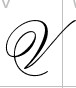
\includegraphics[scale=0.9]{img/v.jpg}
	\caption{Letra V caligrafeada}
\end{figure}
Se eligieron 20 puntos en, los cuales estan en la siguiente tabla y su $t$ correspondiente:
\begin{center}
	\captionof{figure}{Punto inicial: 0.50}
	\begin{longtable}{|c|c|c|} \hline
		$t$   & $x$   & $y$ \\ \hline \hline
		0     & 1.123 & 0.163  \\ \hline
		1/19  & 0.8   & 0.075  \\ \hline
		2/19  & 0.4   & 0.238  \\ \hline
		3/19  & 0.28  & 0.497  \\ \hline
		4/19  & 0.4   & 0.87   \\ \hline
		5/19  & 0.7   & 1.047  \\ \hline
		6/19  & 0.817 & 0.95   \\ \hline
		7/19  & 0.6   & 0.63   \\ \hline
		8/19  & 0.28  & 0.497  \\ \hline
		9/19  & 0.075 & 0.7    \\ \hline
		10/19 & 0.2   & 0.998  \\ \hline
		11/19 & 0.4   & 1.165  \\ \hline
		12/19 & 0.8   & 1.294  \\ \hline
		13/19 & 1.06  & 1.2    \\ \hline
		14/19 & 1     & 0.77   \\ \hline
		15/19 & 0.53  & 0.23   \\ \hline
		16/19 & 0.8   & 0.36   \\ \hline
		17/19 & 1.2   & 0.746  \\ \hline
		18/19 & 1.6   & 1.132  \\ \hline
		1     & 1.84  & 1.289  \\ \hline
		
	\end{longtable}
\end{center}

Obtuvimos el siguiente spline, formado por los siguientes polinomios al armar la función que relaciona $x$ y $t$:
\begin{align*}
S_0(t) & \text{Para x entre} 0.000000000000 \text{ y } 0.05263158 \\
S_0(t) & = 1.12300000-5.43046507(t+0.00000000)+0.00000000(t+0.00000000)^2-255.05910980(t+0.00000000)^3 \\
S_1(t) & \text{Para x entre} 0.052631578947 \text{ y } 0.10526316 \\
S_1(t) & = 0.80000000-7.55006986(t-0.05263158)-40.27249102(t-0.05263158)^2+747.15254902(t-0.05263158)^3 \\
S_2(t) & \text{Para x entre} 0.105263157895 \text{ y } 0.15789474 \\
S_2(t) & = 0.40000000-5.58025549(t-0.10526316)+77.69896409(t-0.10526316)^2-284.88808629(t-0.10526316)^3 \\
S_3(t) & \text{Para x entre} 0.157894736842 \text{ y } 0.21052632 \\
S_3(t) & = 0.28000000+0.23109181(t-0.15789474)+32.71663467(t-0.15789474)^2+118.03979614(t-0.15789474)^3 \\
S_4(t) & \text{Para x entre} 0.210526315789 \text{ y } 0.26315789 \\
S_4(t) & = 0.40000000+4.65588823(t-0.21052632)+51.35449722(t-0.21052632)^2-598.81109828(t-0.21052632)^3 \\
S_5(t) & \text{Para x entre} 0.263157894737 \text{ y } 0.31578947 \\
S_5(t) & = 0.70000000+5.08535526(t-0.26315789)-43.19462356(t-0.26315789)^2-212.61240301(t-0.26315789)^3 \\
S_6(t) & \text{Para x entre} 0.315789473684 \text{ y } 0.36842105 \\
S_6(t) & = 0.81700000-1.22830929(t-0.31578947)-76.76500298(t-0.31578947)^2+413.55171034(t-0.31578947)^3 \\
S_7(t) & \text{Para x entre} 0.368421052632 \text{ y } 0.42105263 \\
S_7(t) & = 0.60000000-5.87211811(t-0.36842105)-11.46736451(t-0.36842105)^2+142.83456165(t-0.36842105)^3 \\
S_8(t) & \text{Para x entre} 0.421052631579 \text{ y } 0.47368421 \\
S_8(t) & = 0.28000000-5.89221829(t-0.42105263)+11.08546102(t-0.42105263)^2+510.37204306(t-0.42105263)^3 \\
S_9(t) & \text{Para x entre} 0.473684210526 \text{ y } 0.52631579 \\
S_9(t) & = 0.07500000-0.48400874(t-0.47368421)+91.67052045(t-0.47368421)^2-709.63773390(t-0.47368421)^3 \\
S_10(t) & \text{Para x entre} 0.526315789474 \text{ y } 0.57894737 \\
S_10(t) & = 0.20000000+3.26825324(t-0.52631579)-20.37754280(t-0.52631579)^2+579.13389254(t-0.52631579)^3 \\
S_11(t) & \text{Para x entre} 0.578947368421 \text{ y } 0.63157895 \\
S_11(t) & = 0.40000000+5.93599577(t-0.57894737)+71.06465076(t-0.57894737)^2-749.52283627(t-0.57894737)^3 \\
S_12(t) & \text{Para x entre} 0.631578947368 \text{ y } 0.68421053 \\
S_12(t) & = 0.80000000+7.18776369(t-0.63157895)-47.28106023(t-0.63157895)^2+86.89745254(t-0.63157895)^3 \\
S_13(t) & \text{Para x entre} 0.684210526316 \text{ y } 0.73684211 \\
S_13(t) & = 1.06000000+2.93294948(t-0.68421053)-33.56040983(t-0.68421053)^2-832.68697387(t-0.68421053)^3 \\
S_14(t) & \text{Para x entre} 0.736842105263 \text{ y } 0.78947368 \\
S_14(t) & = 1.00000000-7.51956159(t-0.73684211)-165.03730044(t-0.73684211)^2+2626.54044295(t-0.73684211)^3 \\
S_15(t) & \text{Para x entre} 0.789473684211 \text{ y } 0.84210526 \\
S_15(t) & = 0.53000000-3.06470311(t-0.78947368)+249.67961160(t-0.78947368)^2-1785.62479792(t-0.78947368)^3 \\
S_16(t) & \text{Para x entre} 0.842105263158 \text{ y } 0.89473684 \\
S_16(t) & = 0.80000000+8.37837403(t-0.84210526)-32.26114596(t-0.84210526)^2+331.96874874(t-0.84210526)^3 \\
S_17(t) & \text{Para x entre} 0.894736842105 \text{ y } 0.94736842 \\
S_17(t) & = 1.20000000+7.74120699(t-0.89473684)+20.15497226(t-0.89473684)^2-433.92019704(t-0.89473684)^3 \\
S_18(t) & \text{Para x entre} 0.947368421053 \text{ y } 1.00000000 \\
S_18(t) & = 1.60000000+6.25679800(t-0.94736842)-48.35874306(t-0.94736842)^2+306.27203941(t-0.94736842)^3
\end{align*}
Y los siguientes polinomios que forman el spline al tener la función que relaciona $t$ con $y$:
\begin{align*}
P_0(t) & \text{Para x entre} 0.000000000000 \text{ y } 0.05263158 \\
P_0(t) & = 0.16300000-2.87433585(t+0.00000000)+0.00000000(t+0.00000000)^2+434.04324177(t+0.00000000)^3 \\
P_1(t) & \text{Para x entre} 0.052631578947 \text{ y } 0.10526316 \\
P_1(t) & = 0.07500000+0.73267170(t-0.05263158)+68.53314344(t-0.05263158)^2-448.60720883(t-0.05263158)^3 \\
P_2(t) & \text{Para x entre} 0.105263157895 \text{ y } 0.15789474 \\
P_2(t) & = 0.23800000+4.21864905(t-0.10526316)-2.29957375(t-0.10526316)^2+297.24059356(t-0.10526316)^3 \\
P_3(t) & \text{Para x entre} 0.157894736842 \text{ y } 0.21052632 \\
P_3(t) & = 0.49700000+6.44673209(t-0.15789474)+44.63315155(t-0.15789474)^2-616.89316541(t-0.15789474)^3 \\
P_4(t) & \text{Para x entre} 0.210526315789 \text{ y } 0.26315789 \\
P_4(t) & = 0.87000000+6.01842257(t-0.21052632)-52.77103246(t-0.21052632)^2+44.04206807(t-0.21052632)^3 \\
P_5(t) & \text{Para x entre} 0.263157894737 \text{ y } 0.31578947 \\
P_5(t) & = 1.04700000+0.82957762(t-0.26315789)-45.81702171(t-0.26315789)^2-94.27710686(t-0.26315789)^3 \\
P_6(t) & \text{Para x entre} 0.315789473684 \text{ y } 0.36842105 \\
P_6(t) & = 0.95000000-4.77673304(t-0.31578947)-60.70288069(t-0.31578947)^2+682.87535939(t-0.31578947)^3 \\
P_7(t) & \text{Para x entre} 0.368421052632 \text{ y } 0.42105263 \\
P_7(t) & = 0.63000000-5.49164547(t-0.36842105)+47.11954448(t-0.36842105)^2+174.96566932(t-0.36842105)^3 \\
P_8(t) & \text{Para x entre} 0.421052631579 \text{ y } 0.47368421 \\
P_8(t) & = 0.49700000+0.92231491(t-0.42105263)+74.74570279(t-0.42105263)^2-360.74703667(t-0.42105263)^3 \\
P_9(t) & \text{Para x entre} 0.473684210526 \text{ y } 0.52631579 \\
P_9(t) & = 0.70000000+5.79238582(t-0.47368421)+17.78564437(t-0.47368421)^2-384.99652265(t-0.47368421)^3 \\
P_10(t) & \text{Para x entre} 0.526315789474 \text{ y } 0.57894737 \\
P_10(t) & = 0.99800000+4.46514182(t-0.52631579)-43.00328026(t-0.52631579)^2+350.59912725(t-0.52631579)^3 \\
P_11(t) & \text{Para x entre} 0.578947368421 \text{ y } 0.63157895 \\
P_11(t) & = 1.16500000+2.85204690(t-0.57894737)+12.35447667(t-0.57894737)^2-379.51298636(t-0.57894737)^3 \\
P_12(t) & \text{Para x entre} 0.631578947368 \text{ y } 0.68421053 \\
P_12(t) & = 1.29400000+0.99867059(t-0.63157895)-47.56862644(t-0.63157895)^2-101.46218180(t-0.63157895)^3 \\
P_13(t) & \text{Para x entre} 0.684210526316 \text{ y } 0.73684211 \\
P_13(t) & = 1.20000000-4.85172927(t-0.68421053)-63.58897093(t-0.68421053)^2+10.29471357(t-0.68421053)^3 \\
P_14(t) & \text{Para x entre} 0.736842105263 \text{ y } 0.78947368 \\
P_14(t) & = 0.77000000-11.45975352(t-0.73684211)-61.96348984(t-0.73684211)^2+1610.41732751(t-0.73684211)^3 \\
P_15(t) & \text{Para x entre} 0.789473684211 \text{ y } 0.84210526 \\
P_15(t) & = 0.23000000-4.59925665(t-0.78947368)+192.31293029(t-0.78947368)^2-1101.94402360(t-0.78947368)^3 \\
P_16(t) & \text{Para x entre} 0.842105263158 \text{ y } 0.89473684 \\
P_16(t) & = 0.36000000+6.48678013(t-0.84210526)+18.32176867(t-0.84210526)^2-42.26723312(t-0.84210526)^3 \\
P_17(t) & \text{Para x entre} 0.894736842105 \text{ y } 0.94736842 \\
P_17(t) & = 0.74600000+8.06413612(t-0.89473684)+11.64799502(t-0.89473684)^2-484.89104392(t-0.89473684)^3 \\
P_18(t) & \text{Para x entre} 0.947368421053 \text{ y } 1.00000000 \\
P_18(t) & = 1.13200000+5.26067539(t-0.94736842)-64.91374876(t-0.94736842)^2+411.12040878(t-0.94736842)^3
\end{align*}

Tenemos que obtuvimos la siguiente gráfica:
\begin{figure}[H]
	\centering
	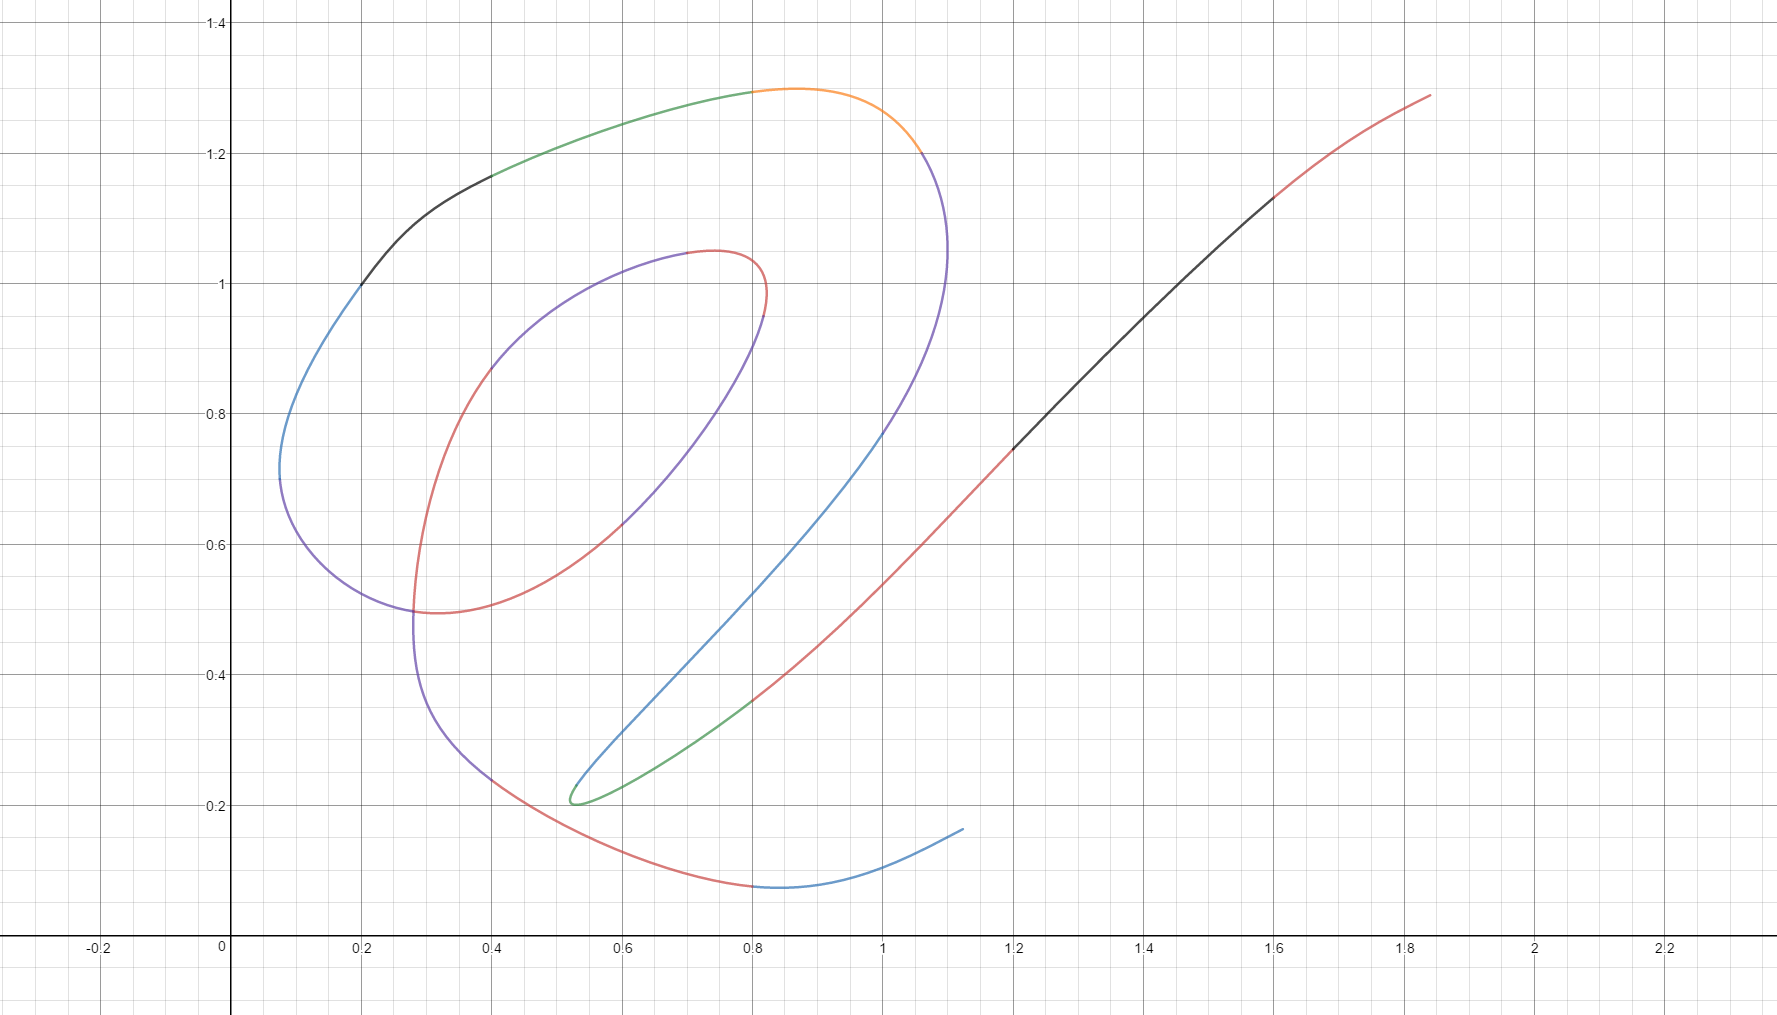
\includegraphics[scale=0.3]{img/4.png}
	\caption{Letra V Con curvas parametricas!}
\end{figure}

Se puede observar con mas detalle, en sl siguiente enlace 
\url{https://www.desmos.com/calculator/dewbwompm8}